\section[Automatisation]{Automatisation du cycle de vie d'une application}

\subsection{Définition}
\begin{frame}{\subsecname}
	\todo{Définition depuis l'intro du mémoire + partie 2.}
\end{frame}

\subsection{Raisons}
\begin{frame}{\subsecname}
	\todo{plusieurs sites à déployer sur NAQ. Soucis de factorisation/ possibilité de pouvoir mettre à disposition du client une version rapidement. Avant : déploiement fait par une ou deux personnes manuellement. Maintenant : déploiement à la demande auto via clic bouton}
\end{frame}

\subsection{Gestion de projet}
\begin{frame}{Partie Financière}
	\begin{columns}[onlytextwidth]
		\column{.47\textwidth}
		\begin{block}{KPI}
			\begin{itemize}
				\item Temps de déploiement réduit
				\item Time to market réduit
				\item PRA
				\item Livrer de la valeur métier plus rapidement
			\end{itemize}
			\note{Exemple sur les projets NAQ, avant déploiements manuels de ~20min/site. Maintenant ~5min par site. Permet de livrer plus rapidment au client, et permet une reprise plus rapide}
		\end{block}
		\column{.47\textwidth}
		\pause
		\begin{figure}
			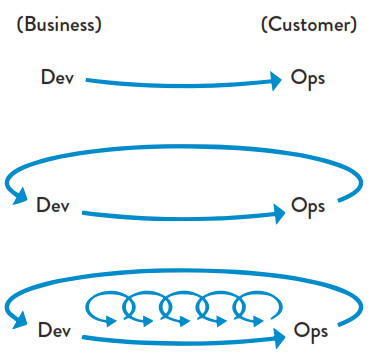
\includegraphics[width=0.9\linewidth]{../img/devops-objective.jpg}
			\caption{Mouvement DevOps}
			\label{fig:devops}
		\end{figure}
	\end{columns}
\end{frame}

\begin{frame}{Organisation}
	\begin{block}{Flux de travail}
		\begin{itemize}
			\item Réduire WIP
			\item Jira
			\item Code review
		\end{itemize}
		\note{Exemple sur les projets NAQ, avant demande qui pouvait trainer plusieurs semaines en attente. Maintenant, on a des demandes qui ne sont pas travaillées tant qu'elles ne sont pas clairemeent définies par le client.}
		\note{Code review qui se met petit à petit en place}
	\end{block}

	\missingfigure{Code review + JIRA}
\end{frame}

\subsection[Développement]{Environnement de développement local}
\begin{frame}{\subsecname}
	IDE
	
	Initialisation ud projet : avant c'était chiant à faire. Maintenant c'est 5 commandes et 10min à peine
\end{frame}

\subsection{Tests}
\begin{frame}{\subsecname}
	Mise en place de POC de test (test unitaire avec mock de composant) \\
	CI test dump de prod pour vérifier que les updates passent bien.
\end{frame}

